% Appendix A

\chapter{Methods} % Main appendix title
\label{appendix:methods} % For referencing this appendix elsewhere, use \ref{AppendixA}


\begin{sidewaystable}[ht]
\resizebox{\textwidth}{!}{%
\begin{tabular}{llllllll}
\hline
\textbf{Lexical Metric} & \textbf{Count} & \textbf{+} & \textbf{-} & \textbf{!} & \textbf{NR} & \textbf{Corr. Symptoms} & \textbf{Classifier Feature} \\ 
\hline
Word Count & 29 &  & \begin{tabular}[c]{@{}l@{}} \cite{mota2014graph, iter2018automatic}; \\ \cite{willits2018evidence, dore2019quantification}; \\ \cite{just2019coherence, just2020modeling}; \\ \cite{panicheva2019semantic}; \textit{\cite{morgan2021natural}}; \\ \textit{\cite{spencer2021lower}}; \cite{voppel2021quantified}; \\ \cite{liang2022widespread, parola2022speech} \end{tabular} & \textit{\begin{tabular}[c]{@{}l@{}} \cite{mota2012speech}; \\ \textit{\cite{gupta2018automated}}; \\ \cite{ryazanskaya2020automated}; \\ \textit{\cite{morgan2021natural}}; \\ \cite{tang2021natural}; \\ \cite{alonso2022language}; \\ \cite{alonso2022progressive}; \\ \cite{schneider2023syntactic}; \\ \textit{\textit{\cite{nettekoven2023semantic}}} \end{tabular}} & \begin{tabular}[c]{@{}l@{}} \cite{koranova2017analyzing}; \\ \textit{\cite{argolo2023burnishing}} \end{tabular} & \textit{\begin{tabular}[c]{@{}l@{}} \textit{\cite{morgan2021natural}}; \\ \cite{minor2023automated} \end{tabular}} & \begin{tabular}[c]{@{}l@{}} \cite{liebenthal2022linguistic}; \\ \cite{tang2022clinical}; \\ \cite{tang2023latent}; \\ \cite{voppel2023semantic} \end{tabular} \\
LD: TTR+ & 8 & \cite{ziv2022morphological} & \begin{tabular}[c]{@{}l@{}} \cite{willits2018evidence, aich2022towards}; \\ \cite{minor2023automated} \end{tabular} & \begin{tabular}[c]{@{}l@{}} \textit{\cite{hitczenko2021understanding}}; \\ \cite{jeong2023exploring}*; \\ \cite{schneider2023syntactic} \end{tabular} &  &  & \begin{tabular}[c]{@{}l@{}} \textit{\cite{rosenstein2015language}}; \\ \cite{kramov2020evaluating}; \\ \cite{liang2022widespread}; \\ \cite{tang2023latent} \end{tabular} \\
LD: Unique Words & 2 &  & \cite{willits2018evidence} & \cite{schneider2023syntactic} &  &  &  \\
LD: Honoré Statistics & 1 &  &  &  &  & \cite{jeong2023exploring} &  \\
SA: Emotion Words & 6 & \cite{mitchell2015quantifying} & \cite{mitchell2015quantifying, aich2022towards} & \cite{mota2022happy} &  & \begin{tabular}[c]{@{}l@{}} \cite{vail2018toward}; \\ \textit{\cite{girard2022computational}}; \\ \cite{minor2023automated} \end{tabular} &  \\
SA: models & 5 &  &  & \textit{\cite{argolo2023burnishing}} &  &  & \begin{tabular}[c]{@{}l@{}} \cite{sarzynska2021detecting, tang2022clinical}; \\ \cite{tang2023latent}; \\ \cite{aich2022towards} \end{tabular} \\
Neologisms, OOV & 2 & \begin{tabular}[c]{@{}l@{}} \cite{just2019coherence}; \\ \cite{just2020modeling} \end{tabular} &  &  &  &  &  \\
Foreign Word Use & 1 &  &  &  &  & \cite{jeong2023exploring} &  \\ 
\hline
\end{tabular}
}
\caption[Summary of the lexical metric results]{\label{tab:method:lexical} Summary of the results reported for the lexical methods used in the reviewed papers. \\ ``+'' indicates significant group difference with \textit{higher} values in the patient population. ``-'' indicates significant group difference with \textit{lower} values in the patient population.  ``!'' indicates absence of significant differences in the metric tested. ``NR'' indicates that the metric is used but results are not reported. ``Corr. Symptoms'' indicates significant correlation with symptom severity in any direction.  ``Classifier Feature'' indicates that the metric is used as a feature in a classifier or latent analysis. The studies on clinical high risk populations are shown in italics. * - no correlation with symptoms.} 
\end{sidewaystable}


\begin{sidewaystable}[ht]
\resizebox{\textwidth}{!}{%
\begin{tabular}{llllllllll}
\hline
\textbf{Syntactic Metric} & \textbf{Count} & \textbf{+} & \textbf{-} & \textbf{!} & \textbf{NR} & \textbf{Corr. Ling. Scale} & \textbf{Corr. Symptoms} & \textbf{No Corr. Symptoms} & \textbf{Classifier Feature} \\ 
\hline
\begin{tabular}[c]{@{}l@{}}POS: det, \\ wh-words\end{tabular} & 10 & \cite{mitchell2015quantifying} & \begin{tabular}[c]{@{}l@{}} \textit{\cite{corcoran2018prediction}}; \\ \cite{sarzynska2021detecting}; \\ \cite{tang2021natural} \end{tabular} & \textit{\begin{tabular}[c]{@{}l@{}} \cite{rezaii2019machine}; \\ \cite{haas2020linking}; \\ \cite{bilgrami2022construct}; \\ \cite{argolo2023burnishing} \end{tabular}} & \textit{\cite{bedi2015automated}} & \textit{\begin{tabular}[c]{@{}l@{}} \cite{corcoran2018prediction}; \\ \cite{bilgrami2022construct} \end{tabular}} & \textit{} & \textit{\begin{tabular}[c]{@{}l@{}} \cite{corcoran2018prediction}; \\ \cite{bilgrami2022construct} \end{tabular}} & \begin{tabular}[c]{@{}l@{}} \textit{\cite{bedi2015automated}}; \\ \cite{tang2021natural} \end{tabular} \\
POS: adj & 12 & \textit{\cite{argolo2023burnishing}} & \begin{tabular}[c]{@{}l@{}}\textit{\cite{corcoran2018prediction}}; \cite{tang2021natural}; \\ \cite{ziv2022morphological} \end{tabular} & \textit{\begin{tabular}[c]{@{}l@{}} \cite{haas2020linking}; \\ \cite{bilgrami2022construct} \end{tabular}} & \begin{tabular}[c]{@{}l@{}}\textit{\cite{bedi2015automated}}; \\ \cite{mitchell2015quantifying}; \\ \textit{\cite{rezaii2019machine}} \end{tabular} & \textit{\cite{corcoran2018prediction}} & \textit{\cite{argolo2023burnishing}} & \textit{\cite{corcoran2018prediction}} & \begin{tabular}[c]{@{}l@{}}\textit{\cite{bedi2015automated}}; \\ \cite{tang2023latent}; \\ \cite{sarzynska2021detecting} \end{tabular} \\
POS: verb & 9 & \cite{mitchell2015quantifying} & \cite{ziv2022morphological} & \begin{tabular}[c]{@{}l@{}}\textit{\cite{haas2020linking}}; \\ \cite{tang2021natural}; \\ \textit{\cite{argolo2023burnishing}} \end{tabular} & \textit{\begin{tabular}[c]{@{}l@{}} \cite{bedi2015automated}; \\ \cite{rezaii2019machine} \end{tabular}} &  &  &  & \begin{tabular}[c]{@{}l@{}} \cite{sarzynska2021detecting}; \\ \cite{tang2022clinical} \end{tabular} \\
POS: pron & 9 & \begin{tabular}[c]{@{}l@{}} \cite{mitchell2015quantifying}; \\ \cite{tang2021natural} \end{tabular} & \textit{\cite{corcoran2018prediction}} & \textit{\begin{tabular}[c]{@{}l@{}} \cite{haas2020linking}; \\ \cite{argolo2023burnishing} \end{tabular}} & \textit{\begin{tabular}[c]{@{}l@{}} \cite{bedi2015automated}; \\ \cite{rezaii2019machine} \end{tabular}} & \textit{\cite{corcoran2018prediction}} & \cite{jeong2023exploring} & \textit{\cite{corcoran2018prediction}} & \cite{sarzynska2021detecting} \\
POS: noun & 7 &  &  & \begin{tabular}[c]{@{}l@{}}\textit{\cite{haas2020linking}}; \\ \cite{tang2021natural}; \\ \cite{ziv2022morphological}; \\ \textit{\cite{argolo2023burnishing}} \end{tabular} & \begin{tabular}[c]{@{}l@{}}\textit{\cite{bedi2015automated}}; \\ \cite{mitchell2015quantifying} \end{tabular} &  &  &  & \cite{sarzynska2021detecting} \\
POS: adv & 6 &  & \cite{tang2021natural, ziv2022morphological} & \textit{\begin{tabular}[c]{@{}l@{}} \cite{haas2020linking}; \\ \cite{argolo2023burnishing} \end{tabular}} & \cite{mitchell2015quantifying} &  &  &  & \cite{sarzynska2021detecting} \\
POS: subconj & 5 & \cite{silva2022syntactic} &  & \begin{tabular}[c]{@{}l@{}}\textit{\cite{haas2020linking}}; \\ \cite{tang2021natural}; \\ \textit{\cite{argolo2023burnishing}} \end{tabular} & \textit{} &  &  &  & \cite{tang2023latent} \\
POS: coorconj & 4 &  &  & \begin{tabular}[c]{@{}l@{}}\textit{\cite{haas2020linking}}; \\ \cite{tang2021natural}; \\ \textit{\cite{argolo2023burnishing}} \end{tabular} &  &  &  &  & \cite{tang2023latent} \\
\begin{tabular}[c]{@{}l@{}}Ambiguous Pronouns, \\ Referential Failures\end{tabular} & 4 & \begin{tabular}[c]{@{}l@{}} \cite{iter2018automatic}; \\ \cite{just2020modeling} \end{tabular} & \cite{morgan2021natural}&  & \textit{\textit{\cite{nettekoven2023semantic}}} & \cite{iter2018automatic} & \cite{iter2018automatic} &  &  \\
Sent. / Unit Length & 16 &  & \begin{tabular}[c]{@{}l@{}} \cite{iter2018automatic,palominos2023coreference}; \\ \textit{\cite{spencer2021lower}}; \cite{tang2021natural}; \\ \textit{\cite{bilgrami2022construct}}; \cite{silva2022syntactic}; \\ \textit{\textit{\cite{nettekoven2023semantic}}}; \\ \cite{schneider2023syntactic} \end{tabular} & \begin{tabular}[c]{@{}l@{}} \cite{liang2022widespread}; \\ \textit{\cite{gupta2018automated}}; \\ \textit{\cite{haas2020linking}}; \\ \textit{\cite{morgan2021natural}} \end{tabular} &  & \begin{tabular}[c]{@{}l@{}} \cite{xu2020centroid}; \\ \textit{\cite{bilgrami2022construct}} \end{tabular} & \begin{tabular}[c]{@{}l@{}} \cite{liebenthal2022linguistic}; \\ \textit{\cite{bilgrami2022construct}}; \\ \cite{silva2022syntactic}; \\ \cite{jeong2023exploring} \end{tabular} &  & \begin{tabular}[c]{@{}l@{}}\textit{\cite{bedi2015automated}}; \\ \cite{tang2023latent} \end{tabular} \\
Sent. Count & 7 & \begin{tabular}[c]{@{}l@{}} \cite{morgan2021natural}; \\ \textit{\textit{\cite{nettekoven2023semantic}}} \end{tabular} & \cite{iter2018automatic} & \begin{tabular}[c]{@{}l@{}}\textit{\cite{gupta2018automated}}; \\ \cite{ryazanskaya2020automated};  \\ \textit{\cite{morgan2021natural}}; \\ \cite{schneider2023syntactic} \end{tabular} & \cite{tang2021natural} &  & \cite{jeong2023exploring} &  &  \\ 
\hline
\end{tabular}
}
\caption[Summary of the syntactic metric results]{\label{tab:method:syntactic} Summary of the results reported for the syntactic methods used in the reviewed papers. \\ ``+'' indicates significant group difference with \textit{higher} values in the patient population. ``-'' indicates significant group difference with \textit{lower} values in the patient population.  ``!'' indicates absence of significant differences in the metric tested. ``NR'' indicates that the metric is used but results are not reported. ``Corr. Symptoms'' indicates significant correlation with symptom severity in any direction. ``No Corr. Symptoms'' indicates absence of significant correlation with symptom severity in any direction. ``Corr. Ling. Scale'' indicates significant correlation with a linguistic symptom scale in any direction.  ``Classifier Feature'' indicates that the metric is used as a feature in a classifier or latent analysis. The studies on clinical high risk populations are shown in italics.  ``POS'' is part-of-speech prefix. ``det'' stands for determiners and determiner pronouns. ``adj'' stands for adjectives. ``pron'' stands for pronoun. ``adv'' stands for adverb. ``Sent.'' stands for sentence.} 
\end{sidewaystable}


\begin{sidewaystable}[ht]
\resizebox{\textwidth}{!}{%
\begin{tabular}{llllllll}
\hline
\textbf{Graph-Based Method} & \textbf{Count} & \textbf{-} & \textbf{!} & \textbf{Corr. Ling. Scale} & \textbf{Corr. Symptoms} & \textbf{No Corr. Symptoms} & \textbf{Classifier Feature} \\
\hline
N & 4 & \cite{nikzad2022does} & \cite{mota2012speech}; \textit{\cite{nettekoven2023semantic}}* &  &  & \cite{mota2012speech} &  \\
E & 6 & \begin{tabular}[c]{@{}l@{}} \cite{mota2014graph, mota2016quantifying}; \\ \cite{mota2017thought, nikzad2022does} \end{tabular} & \cite{mota2012speech}; \textit{\cite{nettekoven2023semantic}}* &  & \begin{tabular}[c]{@{}l@{}} \cite{mota2014graph}; \\ \cite{nikzad2022does} \end{tabular} & \cite{mota2012speech} &  \\
LCC / median CC & 11 & \begin{tabular}[c]{@{}l@{}} \cite{mota2014graph, mota2016quantifying}; \\ \cite{mota2017thought, spencer2021lower}; \\ \cite{morgan2021natural, nikzad2022does}; \\ \cite{nettekoven2023semantic} \end{tabular} & \begin{tabular}[c]{@{}l@{}}\textit{\cite{spencer2021lower, morgan2021natural}}; \\ \textit{\cite{nettekoven2023semantic}}*; \textit{\cite{argolo2023burnishing}} \end{tabular} & \begin{tabular}[c]{@{}l@{}}\textit{\cite{spencer2021lower}}; \\ \textit{\cite{morgan2021natural}}; \\ \textit{\cite{nettekoven2023semantic}}**\end{tabular} & \begin{tabular}[c]{@{}l@{}} \cite{mota2014graph}; \\ \cite{mota2016quantifying} \end{tabular} & \begin{tabular}[c]{@{}l@{}} \cite{mota2012speech}; \\ \textit{\cite{nettekoven2023semantic}} \end{tabular} & \begin{tabular}[c]{@{}l@{}} \cite{mota2017thought}; \\ \cite{mota2022happy} \end{tabular} \\
LSC & 11 & \begin{tabular}[c]{@{}l@{}} \cite{mota2014graph, mota2016quantifying}; \\ \cite{mota2017thought, spencer2021lower}; \\ \cite{morgan2021natural} \end{tabular} & \begin{tabular}[c]{@{}l@{}} \textit{\cite{spencer2021lower, morgan2021natural}}; \\ \cite{nikzad2022does}; \textit{\cite{argolo2023burnishing}}*\end{tabular} & \begin{tabular}[c]{@{}l@{}}\textit{\cite{spencer2021lower}}; \\ \textit{\cite{morgan2021natural}}; \\ \cite{nikzad2022does} \end{tabular} & \begin{tabular}[c]{@{}l@{}} \cite{mota2014graph}; \\ \cite{mota2016quantifying}; \\ \cite{nikzad2022does} \end{tabular} & \begin{tabular}[c]{@{}l@{}} \cite{mota2012speech}; \\ \textit{\cite{argolo2023burnishing}}*\end{tabular} & \begin{tabular}[c]{@{}l@{}} \cite{mota2017thought}; \\ \cite{mota2022happy}; \\ \cite{tang2022clinical}; \\ \textit{\cite{argolo2023burnishing}} \end{tabular} \\
LCCz/LCCr & 5 & \cite{spencer2021lower, morgan2021natural} & \begin{tabular}[c]{@{}l@{}} \cite{mota2016quantifying, mota2017thought}; \\ \textit{\cite{spencer2021lower, morgan2021natural}} \end{tabular} & \begin{tabular}[c]{@{}l@{}}\textit{\cite{spencer2021lower}}; \\ \textit{\cite{morgan2021natural}} \end{tabular} & \cite{mota2016quantifying} &  &  \\
LSCz/LSCr & 5 & \begin{tabular}[c]{@{}l@{}} \cite{mota2016quantifying, mota2017thought}; \\ \cite{spencer2021lower, morgan2021natural}; \\ \cite{nikzad2022does} \end{tabular} & \textit{\cite{spencer2021lower, morgan2021natural}} & \begin{tabular}[c]{@{}l@{}}\textit{\cite{spencer2021lower}}; \\ \textit{\cite{morgan2021natural}}; \\ \cite{nikzad2022does} \end{tabular} & \begin{tabular}[c]{@{}l@{}} \cite{mota2016quantifying}; \\ \cite{nikzad2022does} \end{tabular} &  & \begin{tabular}[c]{@{}l@{}} \cite{mota2017thought}; \\ \cite{mota2022happy} \end{tabular} \\
ASP & 6 & \cite{mota2014graph} & \begin{tabular}[c]{@{}l@{}} \cite{mota2012speech, tang2022clinical}; \\ \cite{nikzad2022does}; \textit{\cite{argolo2023burnishing}} \end{tabular} &  & \cite{nikzad2022does} & \cite{mota2012speech} & \begin{tabular}[c]{@{}l@{}} \cite{tang2022clinical}; \\ \textit{\cite{argolo2023burnishing}} \end{tabular} \\
density & 5 & \cite{nikzad2022does} & \begin{tabular}[c]{@{}l@{}} \cite{mota2012speech, mota2014graph}; \\ \textit{\cite{argolo2023burnishing}}*\end{tabular} & \cite{nikzad2022does} & \cite{nikzad2022does} & \cite{mota2012speech} & \begin{tabular}[c]{@{}l@{}}\cite{tang2022clinical}; \\ \textit{\cite{argolo2023burnishing}} \end{tabular} \\
diameter & 5 & \cite{mota2014graph} & \cite{mota2012speech, nikzad2022does} & \cite{nikzad2022does} &  & \cite{mota2012speech} & \cite{tang2022clinical} \\
ATD & 4 & \cite{mota2014graph} & \cite{mota2012speech}* &  &  & \cite{mota2012speech} & \cite{tang2022clinical} \\
AWD & 1 & \cite{nikzad2022does} &  & \cite{nikzad2022does} &  &  &  \\
Largest Clique & 2 &  &  &  &  &  & \begin{tabular}[c]{@{}l@{}}\cite{tang2022clinical}; \\ \cite{tang2023latent} \end{tabular} \\
Clustering Coefficient & 1 &  &  &  &  &  & \cite{tang2023latent}\\ 
\hline
\end{tabular}
}
\caption[Summary of the graph-based metric results]{\label{tab:method:graph} Summary of the results reported for the graph-based methods used in the reviewed papers. \\ ``-'' indicates significant group difference with \textit{lower} values in the patient population.  ``!'' indicates absence of significant differences in the metric tested. ``NR'' indicates that the metric is used but results are not reported. ``Corr. Symptoms'' indicates significant correlation with symptom severity in any direction. ``No Corr. Symptoms'' indicates absence of significant correlation with symptom severity in any direction. ``Corr. Ling. Scale'' indicates significant correlation with a linguistic symptom scale in any direction.  ``Classifier Feature'' indicates that the metric is used as a feature in a classifier or latent analysis. The studies on clinical high risk populations are shown in italics. Some studies report both for SZ and CHR and are reported twice. ``*'' means the metric was insignificant after corrections for verbosity. ``**'' means the metric was insignificant after correcting for multiple comparisons. ``N'' stands for number of nodes. ``E'' stands for number of edges. ``LCC'' stands for largest connected component. ``CC'' stands for connected component. ``LSC'' stands for largest strongly connected component. ``LCCz/LCCr'' stands for z-score or randomness of the largest connected component. ``LSCz/LSCr'' stands for z-score or randomness of the largest strongly connected component. ``ASP'' stands for average shortest path. ``ATD'' stands for average total degree. ``AWD'' stands for average weighted degree.} 
\end{sidewaystable}


\begin{sidewaystable}[ht]
\resizebox{\textwidth}{!}{%
\begin{tabular}{llllllll}
\hline
\textbf{LM-Based Method} & \textbf{Count} & \textbf{+} & \textbf{-} & \textbf{!} & \textbf{Corr. Ling. Scale} & \textbf{Corr. Symptoms} & \textbf{No Corr. Symptoms} \\ \hline
Moving Window Coherence & 8 & \begin{tabular}[c]{@{}l@{}} \cite{panicheva2020corpus} (min); \\ \cite{alonso2022language}; \\ \cite{alonso2022progressive}; \\ \cite{voppel2021quantified} (var); \\ \cite{voppel2023semantic} (var)\end{tabular} & \begin{tabular}[c]{@{}l@{}} \cite{bar2019semantic}; \\ \cite{panicheva2020corpus} (max); \\ \cite{parola2022speech} (Ch)\end{tabular} & \begin{tabular}[c]{@{}l@{}} \cite{dore2019quantification}; \\ \cite{parola2022speech} (D, G)\end{tabular} &  &  &  \\
Word-Based Coherence & 5 & \cite{parola2022speech} (D) & \begin{tabular}[c]{@{}l@{}}\cite{bar2019semantic}; \\ \cite{parola2022speech} (Ch, G)\end{tabular} & \begin{tabular}[c]{@{}l@{}} \cite{liebenthal2022linguistic}; \\ \textit{\cite{argolo2023burnishing}} \end{tabular} & \begin{tabular}[c]{@{}l@{}}\cite{xu2020centroid}; \\ \cite{xu2022fully} \end{tabular} &  &  \\
K-Inter Word Similarity & 3 &  & \textit{\cite{corcoran2018prediction}} & \begin{tabular}[c]{@{}l@{}}\cite{parola2022speech} (?); \\ \textit{\cite{argolo2023burnishing}} \end{tabular} &  &  & \textit{\cite{corcoran2018prediction}} \\
All word Similarity & 3 &  &  &  &  & \cite{alonso2022progressive} &  \\
Vector Magnitude & 2 &  & \textit{} & \textit{\begin{tabular}[c]{@{}l@{}} \textit{\cite{rezaii2019machine}}; \\ \cite{liebenthal2022linguistic}\end{tabular}} & \textit{} &  &  \\
\begin{tabular}[c]{@{}l@{}}Word-Based Centroid Global Coherence \&\\ Word-Based Cumulative Centroid Global Coherence\end{tabular} & 2 &  & \textit{} &  & \begin{tabular}[c]{@{}l@{}} \cite{xu2020centroid}; \\ \cite{xu2022fully} \end{tabular} &  &  \\ 
\hline
\end{tabular}
}
\caption[Summary of the word-embedding based metric results]{\label{tab:method:word-embedding} Summary of the results reported for the word embedding-based metrics used in the reviewed papers. \\ ``-'' indicates significant group difference with \textit{lower} values in the patient population.  ``!'' indicates absence of significant differences in the metric tested. ``Corr. Symptoms'' indicates significant correlation with symptom severity in any direction. ``No Corr. Symptoms'' indicates absence of significant correlation with symptom severity in any direction. ``Corr. Ling. Scale'' indicates significant correlation with a linguistic symptom scale in any direction.  The studies on clinical high risk populations are shown in italics. Some studies report both for several languages - ``Ch'' stands for Chinese, ``D'' - for Danish, and ``G'' - for German. ``min'' indicates that minimum values are reported, ``max'' stands for maximum values, and ``var'' - for variance.}
\end{sidewaystable}



\begin{sidewaystable}[ht]
\resizebox{\textwidth}{!}{%
\begin{tabular}{llllllllll}
\hline
\textbf{LM-Based Method} & \textbf{Count} & \textbf{+} & \textbf{-} & \textbf{!} & \textbf{NR} & \textbf{Corr. Ling. Scale} & \textbf{Corr. Symptoms} & \textbf{No Corr. Symptoms} & \textbf{Classifier Feature} \\ 
\hline
(First-Order) Coherence & 22 &  & \begin{tabular}[c]{@{}l@{}} \cite{iter2018automatic}; \\ \cite{just2019coherence}; \\ \cite{ryazanskaya2020thesis}; \\ \textit{\cite{morgan2021natural}} \end{tabular} & \begin{tabular}[c]{@{}l@{}} \textit{\cite{haas2020linking}}; \\ \cite{just2020modeling}; \\ \textit{\cite{hitczenko2021understanding}}; \\ \cite{parola2022speech}; \\ \textit{\cite{bilgrami2022construct}} \end{tabular} & \textit{\cite{nettekoven2023semantic}} & \begin{tabular}[c]{@{}l@{}}\cite{xu2020centroid}; \\ \cite{xu2022fully};\\ \textit{\cite{bilgrami2022construct}}\end{tabular} & \begin{tabular}[c]{@{}l@{}} \cite{ryazanskaya2020thesis}; \\ \cite{just2023validation} \end{tabular} & \begin{tabular}[c]{@{}l@{}}\textit{\cite{bedi2015automated}}; \\ \cite{iter2018automatic}; \\ \textit{\cite{haas2020linking}}; \\ \textit{\cite{hitczenko2021understanding}}; \\ \cite{parola2022speech} (?); \\ \textit{\cite{bilgrami2022construct}}\end{tabular} & \begin{tabular}[c]{@{}l@{}}\textit{\cite{bedi2015automated}; \cite{rosenstein2015language}}; \\ \cite{iter2018automatic}; \cite{just2020modeling}; \\ \cite{ryazanskaya2020automated}; \\ \cite{sarzynska2021detecting}; \\ \cite{tang2022clinical, tang2023latent}\end{tabular} \\
Second order Coherence & 3 &  & \cite{parola2022speech} &  &  &  &  &  & \begin{tabular}[c]{@{}l@{}}\textit{\cite{bedi2015automated}}; \\ \cite{sarzynska2021detecting}\end{tabular} \\
Repetitiveness & 1 &  &  & \textit{\cite{morgan2021natural}} &  &  &  &  &  \\
Group Global Coherence & 4 &  & \cite{ryazanskaya2020thesis} &  &  & \begin{tabular}[c]{@{}l@{}} \cite{elvevaag2007quantifying}; \\ \cite{elvevaag2010automated}; \\ \cite{ryazanskaya2020automated} \end{tabular} & \cite{ryazanskaya2020thesis} &  &  \\
Gold Standard Global Coherence & 3 &  & \textit{\cite{morgan2021natural}} &  & \textit{\cite{nettekoven2023semantic}} & \cite{ryazanskaya2020automated} &  &  &  \\
Centroid Global Coherence & 4 &  & \cite{ryazanskaya2020thesis} &  &  & \begin{tabular}[c]{@{}l@{}}\cite{xu2020centroid}; \\ \cite{xu2022fully}\end{tabular} & \begin{tabular}[c]{@{}l@{}}\cite{ryazanskaya2020thesis}; \\ \cite{just2023validation}\end{tabular} &  &  \\
Cumulative Centroid Global Coherence & 3 &  & \cite{ryazanskaya2020thesis} &  &  & \begin{tabular}[c]{@{}l@{}}\cite{xu2020centroid}; \\ \cite{xu2022fully}\end{tabular} & \cite{ryazanskaya2020thesis} &  &  \\
Slope Tangentiality & 9 & \begin{tabular}[c]{@{}l@{}} \cite{iter2018automatic}; \\ \cite{tang2021natural} \end{tabular} &  & \begin{tabular}[c]{@{}l@{}} \cite{koranova2017analyzing}; \cite{just2019coherence}; \\ \cite{dore2019quantification}; \textit{\cite{hitczenko2021understanding}}; \\ \cite{morgan2021natural}\end{tabular} &  & \cite{elvevaag2007quantifying} & \textit{} & \begin{tabular}[c]{@{}l@{}} \cite{dore2019quantification}; \\ \textit{\cite{hitczenko2021understanding}}; \\ \cite{morgan2021natural}\end{tabular} &  \\
Q-similarity Tangentiality & 4 &  & \textit{\cite{morgan2021natural}} & \cite{koranova2017analyzing, just2019coherence} & \textit{\cite{nettekoven2023semantic}} &  &  &  &  \\ 
\hline
\end{tabular}
}
\caption[Summary of the phrase-embedding based metric results]{\label{tab:method:sent-embedding} Summary of the results reported for the phrase embedding-based metrics used in the reviewed papers. \\ ``-'' indicates significant group difference with \textit{lower} values in the patient population.  ``!'' indicates absence of significant differences in the metric tested. ``Corr. Symptoms'' indicates significant correlation with symptom severity in any direction. ``No Corr. Symptoms'' indicates absence of significant correlation with symptom severity in any direction. ``Corr. Ling. Scale'' indicates significant correlation with a linguistic symptom scale in any direction.  The studies on clinical high risk populations are shown in italics. ``?'' indicates that the information in the article only allows for a presumable placement of the article.}
\end{sidewaystable}


\begin{sidewaystable}[ht]
\resizebox{\textwidth}{!}{%
\begin{tabular}{llllllll}
\hline
\textbf{LM-Based Method} & \textbf{Count} & \textbf{+} & \textbf{!} & \textbf{Corr. Ling. Scale} & \textbf{Corr. Symptoms} & \textbf{No Corr. Symptoms} & \textbf{Classifier Feature} \\ \hline
Perplexity / Surprisal & 5 &  \cite{srivastava2022increased} & \begin{tabular}[c]{@{}l@{}} \cite{mitchell2015quantifying}; \\ \textit{\cite{srivastava2022increased}}; \\ \cite{jeong2023exploring}\end{tabular} & \cite{jeong2023exploring} & \begin{tabular}[c]{@{}l@{}}\cite{vail2018toward}; \\ \cite{girard2022computational}; \\ \cite{jeong2023exploring}\end{tabular} & \textit{} & \textit{} \\
Next-Sentence Prediction & 3 &  & \textit{\begin{tabular}[c]{@{}l@{}} \textit{\cite{hitczenko2021understanding}}; \\ \cite{tang2021natural}\end{tabular}} & \cite{jeong2023exploring} & \cite{jeong2023exploring} & \cite{tang2021natural} & \textit{} \\
Non-Fine-Tuned Classifier & 3 &  & \textit{} &  &  &  & \begin{tabular}[c]{@{}l@{}} \cite{elvevaag2010automated}; \\ \textit{\cite{rosenstein2015language}}; \\ \textit{\cite{srivastava2022p473}}\end{tabular} \\
Fine-Tuned Classifier & 3 &  &  &  &  &  & \begin{tabular}[c]{@{}l@{}} \cite{wouts2021belabbert}; \\ \cite{aich2022towards}; \\ \cite{shriki2022masking}\end{tabular} \\ \hline
\end{tabular}
}
\caption[Summary of the LM-based feature metric results]{\label{tab:method:feature} Summary of the results reported for the LM-based feature metrics used in the reviewed papers. \\ ``+'' indicates significant group difference with \textit{higher} values in the patient population.  ``!'' indicates absence of significant differences in the metric tested. ``Corr. Symptoms'' indicates significant correlation with symptom severity in any direction. ``No Corr. Symptoms'' indicates absence of significant correlation with symptom severity in any direction. ``Corr. Ling. Scale'' indicates significant correlation with a linguistic symptom scale in any direction.  The studies on clinical high risk populations are shown in italics.}
\end{sidewaystable}

\begin{sidewaystable}[ht]
\resizebox{\textwidth}{!}{%
\begin{tabularx}{\linewidth}{l@{\hspace{1em}}l@{\hspace{1em}}X@{}}
\hline
\textbf{LM} & \textbf{Count} & \textbf{Papers} \\ 
\hline
LSA & 10 & \cite{elvevaag2007quantifying, elvevaag2010automated, bedi2015automated, rosenstein2015language, iter2018automatic, xu2020centroid, haas2020linking, hitczenko2021understanding, tang2022clinical, tang2023latent} \\
Word2Vec & 24 & \cite{koranova2017analyzing, iter2018automatic, rezaii2019machine, just2019coherence, bar2019semantic, panicheva2019semantic, dore2019quantification, ryazanskaya2020thesis, ryazanskaya2020automated, xu2020centroid, hitczenko2021understanding, morgan2021natural, sarzynska2021detecting, voppel2021quantified, corona2022assessing, liebenthal2022linguistic, parola2022speech, tang2021natural, xu2022fully, argolo2023burnishing, just2023validation, nettekoven2023semantic, tang2023latent, voppel2023semantic} \\
GloVe & 8 & \cite{iter2018automatic, just2019coherence, hitczenko2021understanding, alonso2022language, alonso2022progressive, tang2022clinical, just2020modeling, tang2023latent} \\
BERT & 10 & \cite{ryazanskaya2020thesis, hitczenko2021understanding, tang2021natural, wouts2021belabbert, aich2022towards, bilgrami2022construct, srivastava2022p473, shriki2022masking, xu2022fully, jeong2023exploring} \\
ELMo & 4 & \cite{ryazanskaya2020thesis, hitczenko2021understanding, sarzynska2021detecting, srivastava2022increased} \\
sent2vec & 3 & \cite{iter2018automatic, just2019coherence, hitczenko2021understanding}\\
Trigram backoff & 3 & \cite{mitchell2015quantifying, vail2018toward, girard2022computational} \\ 
\hline
\end{tabularx}
}
\caption[Models used for LM-based metrics]{\label{tab:method:LM-models} Models used for LM-based metrics.}
\end{sidewaystable}


\begin{sidewaystable}[ht]
\resizebox{\textwidth}{!}{%
\begin{tabularx}{\linewidth}{l@{\hspace{1em}}l@{\hspace{1em}}X@{}}
\hline
\textbf{Averaging} & \textbf{Count} & \textbf{Papers} \\ 
\hline
Mean & 28 & \cite{bedi2015automated, mitchell2015quantifying, corcoran2018prediction, bar2019semantic, dore2019quantification, just2019coherence, panicheva2019semantic, haas2020linking, just2020modeling, ryazanskaya2020thesis, xu2020centroid, hitczenko2021understanding, voppel2021quantified, morgan2021natural, sarzynska2021detecting, alonso2022language, alonso2022progressive, corona2022assessing, girard2022computational, liebenthal2022linguistic, srivastava2022increased, srivastava2022p473, tang2022clinical, argolo2023burnishing, jeong2023exploring, just2023validation, nettekoven2023semantic, tang2023latent, voppel2023semantic} \\
Min & 14 & \cite{bedi2015automated, corcoran2018prediction, iter2018automatic, panicheva2019semantic, haas2020linking, ryazanskaya2020thesis, xu2020centroid, morgan2021natural, sarzynska2021detecting, voppel2021quantified, bilgrami2022construct, corona2022assessing, xu2022fully, voppel2023semantic} \\
Max & 11 & \cite{bedi2015automated, corcoran2018prediction, panicheva2019semantic, haas2020linking, ryazanskaya2020thesis, morgan2021natural, bilgrami2022construct, corona2022assessing, argolo2023burnishing, just2023validation, voppel2023semantic} \\
SD / Variance & 9 & \cite{bedi2015automated, corcoran2018prediction, panicheva2019semantic, haas2020linking, hitczenko2021understanding, sarzynska2021detecting, voppel2021quantified, corona2022assessing, voppel2023semantic} \\
Median & 4 & \cite{bedi2015automated, sarzynska2021detecting, corona2022assessing, parola2022speech} \\
Percentiles & 2 & \cite{corcoran2018prediction, panicheva2019semantic} \\
IQR & 1 & \cite{parola2022speech} \\ 
\hline
\end{tabularx}
}
\caption[Averaging methods used for LM-based metrics]{\label{tab:method:score-averaging} Averaging methods used for LM-based metrics.}
\end{sidewaystable}


\begin{sidewaystable}[ht]
\resizebox{\textwidth}{!}{%
\begin{tabularx}{\linewidth}{l@{\hspace{1em}}l@{\hspace{1em}}X@{}}
\hline
\textbf{Sent. Averaging} & \multicolumn{1}{l}{\textbf{Count}} & \textbf{Papers} \\ 
\hline
Mean & 23 & \cite{elvevaag2007quantifying, elvevaag2010automated, bedi2015automated, rosenstein2015language, corcoran2018prediction, bar2019semantic, dore2019quantification, panicheva2019semantic, rezaii2019machine, haas2020linking, hitczenko2021understanding, tang2021natural, sarzynska2021detecting, voppel2021quantified, alonso2022language, alonso2022progressive, corona2022assessing, liebenthal2022linguistic, parola2022speech, tang2022clinical, just2023validation, tang2023latent, voppel2023semantic} \\
IDF & 8 & \cite{iter2018automatic, just2019coherence, just2020modeling, ryazanskaya2020automated, xu2020centroid, hitczenko2021understanding, xu2022fully, tang2023latent} \\
SIF & 6 & \cite{iter2018automatic, just2019coherence, ryazanskaya2020thesis, hitczenko2021understanding, morgan2021natural, nettekoven2023semantic} \\
Sum & 1 & \cite{xu2020centroid} \\ 
\hline
\end{tabularx}
}
\caption[Sentence averaging methods used for word embedding-based metrics]{\label{tab:method:word-embedding-averaging} Sentence averaging methods used for word embedding-based metrics.}
\end{sidewaystable}


\begin{figure}[ht!]
    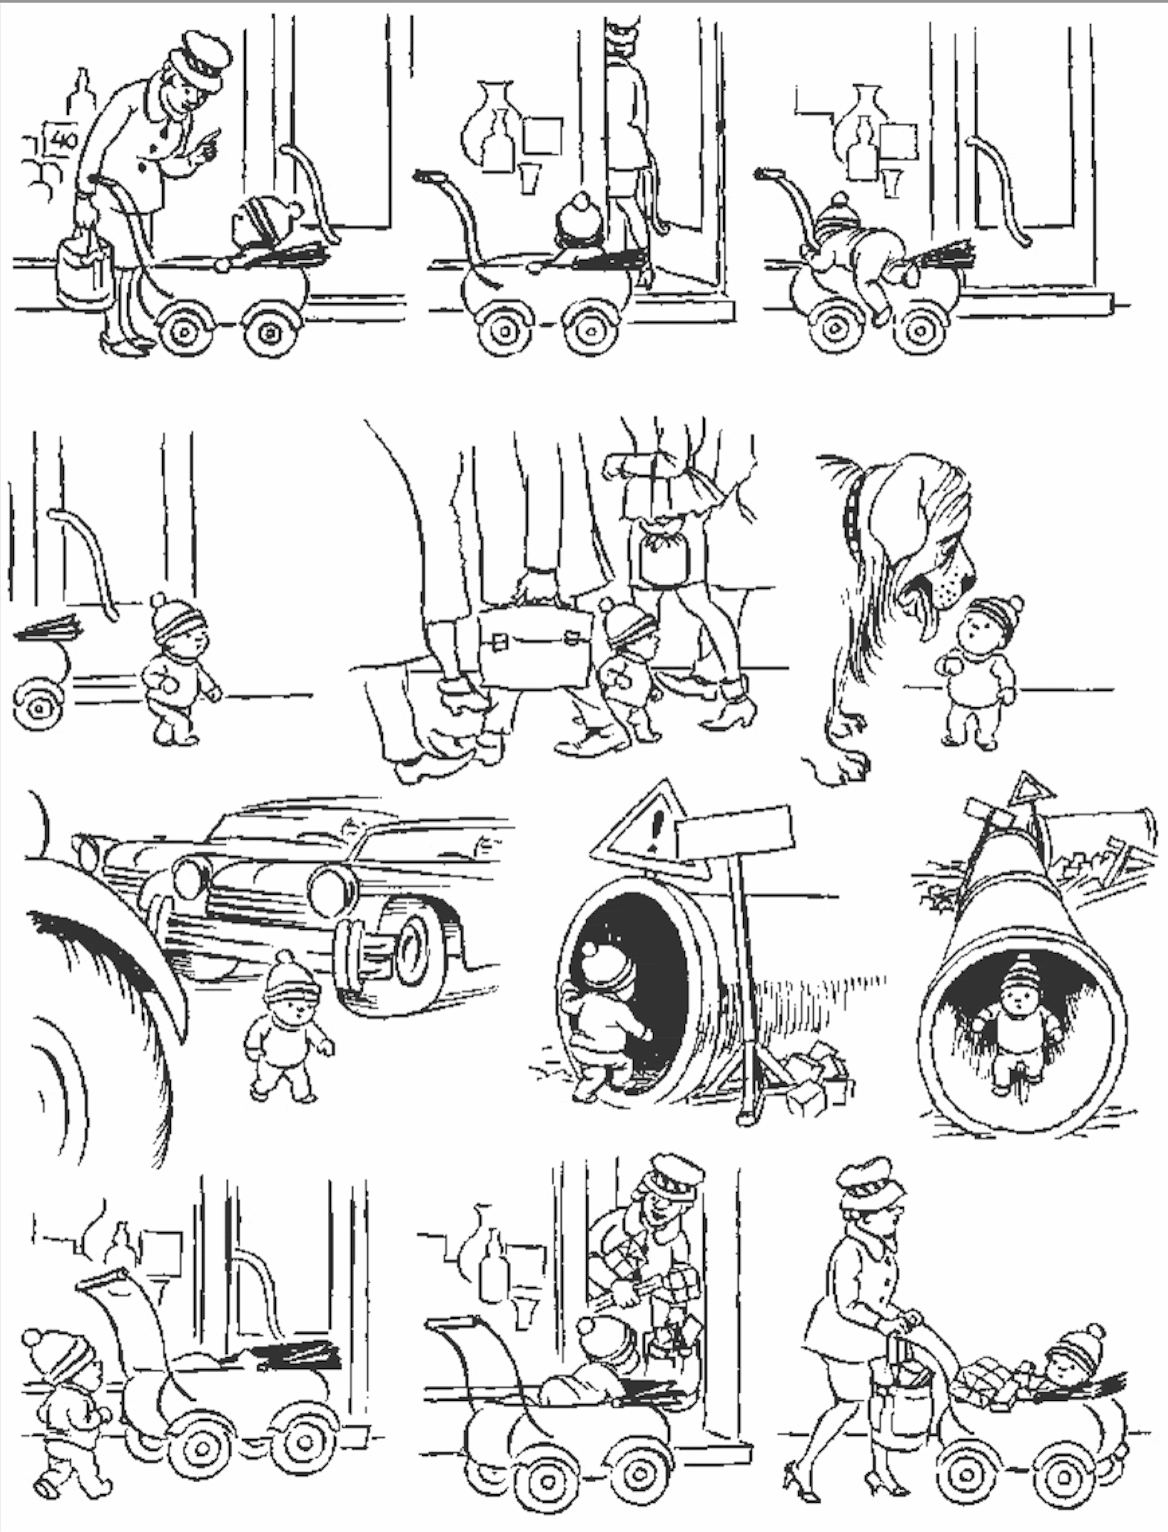
\includegraphics[width=\textwidth, center]{Figures/elicitation/adventure.png} 
\captionsetup{width=\textwidth}
\caption[Tasks: Adventure]{\label{fig:tasks:ad} The image used to elicit adventure task.}
\end{figure}

\begin{figure}[ht!]
    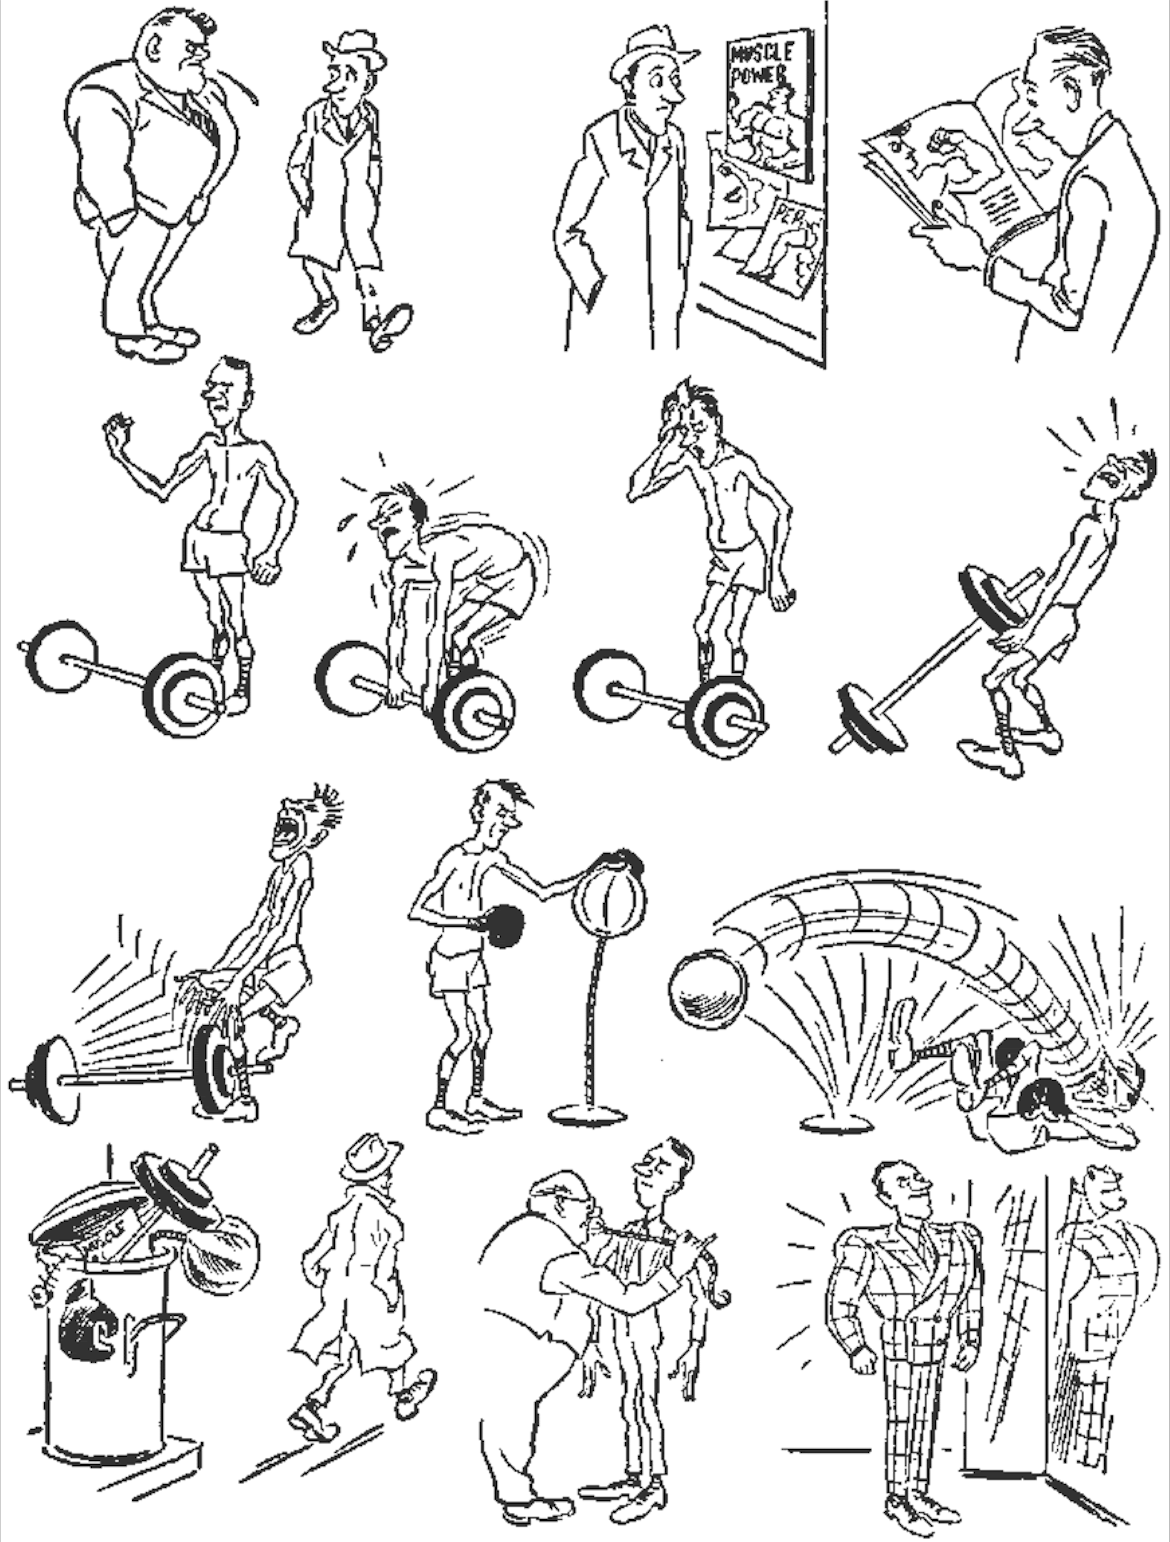
\includegraphics[width=\textwidth, center]{Figures/elicitation/sportsman.png} 
\captionsetup{width=\textwidth}
\caption[Tasks: Sportsman]{\label{fig:tasks:sp} The image used to elicit sportsman task.}
\end{figure}

\begin{figure}[ht!]
    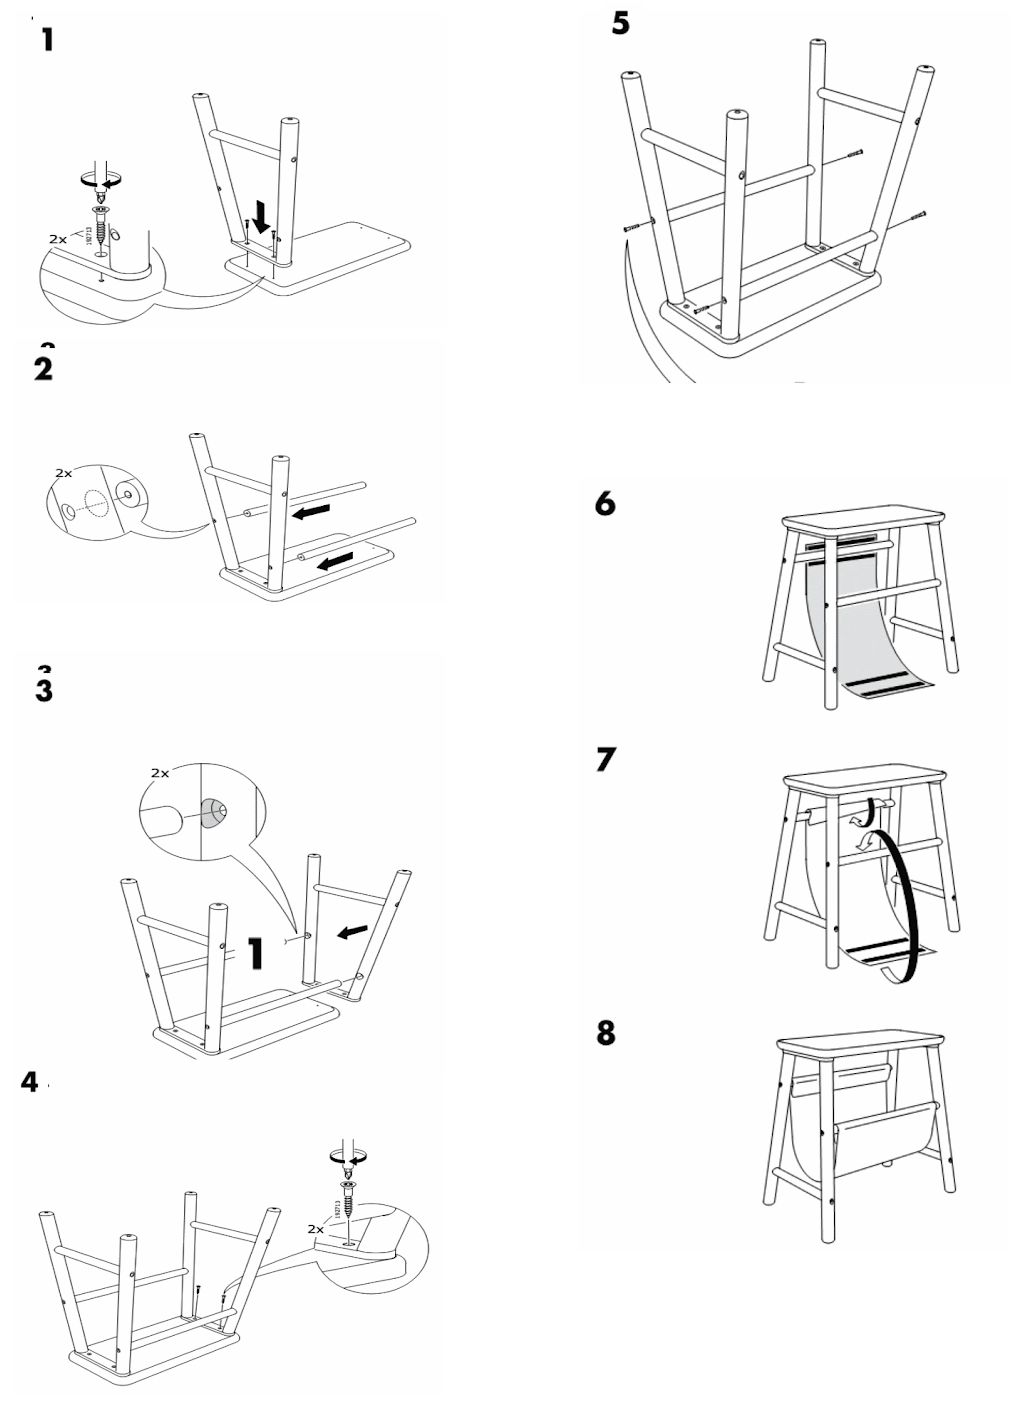
\includegraphics[width=\textwidth, center]{Figures/elicitation/chair.png} 
\captionsetup{width=\textwidth}
\caption[Tasks: Chair]{\label{fig:tasks:ch} The image used to elicit chair task.}
\end{figure}